\documentclass[14pt]{elegantbook}

\newcommand{\CN}{BIOS 7650\\[0.5cm] Stat Learning in Data Analysis}
\newcommand{\Ti}{Homework 1}
\newcommand{\Pf}{Dr. Li}
\newcommand{\FN}{Zehao}
\newcommand{\LN}{Wang}
\usepackage[fontsize=14pt]{fontsize}

\definecolor{LightGray}{gray}{0.9}
\usepackage{minted}

\usepackage{enumitem}
\renewcommand{\chaptername}{Homework}
\begin{document}
\begin{titlepage}
    \begin{center}    
    
\includegraphics[width=0.6\textwidth]{Tulane.png}\\[1cm]    
    
    \textsc{\Huge \CN}\\[0.5cm]
    \textsc{\large \Pf}\\[1.0cm]
    
    \textsc{\LARGE \Ti}\\[0.5cm]
    \textsc{\large \LN, \FN}\\
    {Master student in Statistics of Math Dept.}
    
    % Author and supervisor
    
    \vfill
    
    % Bottom of the page
    {\Large \emph{\today}}
    
    \end{center}
\end{titlepage}

\thispagestyle{empty}
\tableofcontents
\chapter{}

\begin{exercise*}[5]
    What are the advantages and disadvantages of a very flexible (versus a less flexible) approach for regression or classification? Under what circumstances might a more flexible approach be preferred to a less flexible approach? When might a less flexible approach be preferred? 
\end{exercise*}

\begin{solution}
    The advantages of the flexible approach are that it can fit more complex data. But the flexible models are less interpretable. When we want the model to fit the data more accurately but don't care about the interpretability, we can use the flexible approach. When we want the model to be more interpretable, or we need to focus on some parameters in the model, we can use the less flexible approach. 
\end{solution}

\begin{exercise*}[6]
    Describe the differences between a parametric and a non-parametric statistical learning approach. What are the advantages of a parametric approach to regression or classification (as opposed to a non-parametric approach)? What are its disadvantages? 
\end{exercise*}

\begin{solution}
    The parametric approach assumes that the data is generated by a certain distribution. The non-parametric approach doesn't assume the distribution of the data. The parametric approach is more interpretable. But the non-parametric approach is more flexible. 
\end{solution}

\begin{exercise*}[7]
    The table below provides a training data set containing six observations, three predictors, and one qualitative response variable.
    \begin{figure}[h]
        \centering
        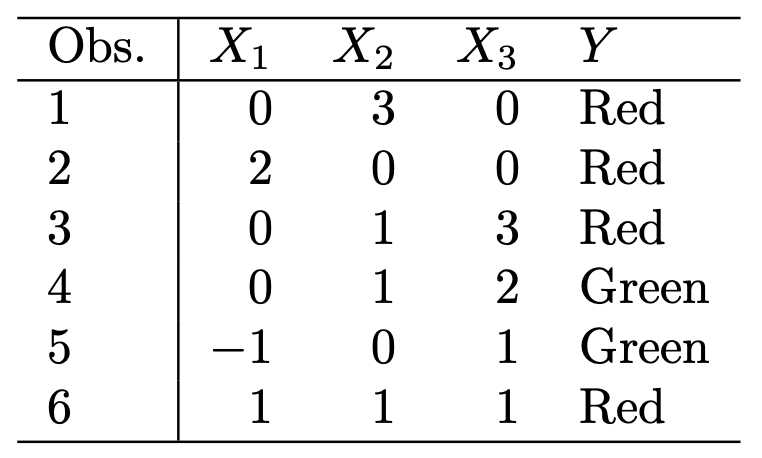
\includegraphics[width=0.5\textwidth]{HW1.png}
    \end{figure}
    Suppose we wish to use this data set to make a prediction for $Y$ when $X_1 = X_2 = X_3 = 0$ using K-nearest neighbors. 
    \begin{enumerate}[(a)]
        \item Compute the Euclidean distance between each observation and the test point,$X_1 =X_2 =X_3 =0$. 
        \item What is our prediction with $K = 1$? Why?
        \item What is our prediction with $K = 3$? Why?
        \item If the Bayes decision boundary in this problem is highly non-linear, then would we expect the best value for K to be large or small? Why?
    \end{enumerate}
\end{exercise*}

\begin{solution}
    \begin{enumerate}[(a)]
        \item $d_1 = \sqrt{0^2 + 3^2 + 0^2} = 3$, 
        
        $d_2 = \sqrt{2^2 + 0^2 + 0^2} = 2$, 
        
        $d_3 = \sqrt{0^2 + 1^2 + 3^2} = \sqrt{10}$, 
        
        $d_4 = \sqrt{1^2 + 2^2 + 0^2} = \sqrt{5}$, 
        
        $d_5 = \sqrt{(-1)^2 + 0^2 + 1^2} = \sqrt{2}$, 
        
        $d_6 = \sqrt{1^2 + 1^2 + 1^2} = \sqrt{3}$.
        \item $d_5=\sqrt{2}$ is the smallest one, so the prediction is $Y = Green$. 
        \item $d_5=\sqrt{2}, d_6=\sqrt{3}, d_2=2$, they are the three smallest ones. So the prediction is $Y = Red$. 
        
        \item Small. The Bayes decision boundary is highly non-linear, and in order to be flexible, K couldn't be large. 
    \end{enumerate}
\end{solution}

\begin{exercise*}
    Think of two situations in your life/study/research which could be a statistical learning  problem. Indicate whether/why it is a supervised or unsupervised learning. (This question will NOT graded by “right” or “wrong”: instead, just graded for whether you think over and answer this question. So feel free to raise any situations that you think or you'd like to apply statistical learning methods.) 
\end{exercise*}

\begin{solution}
    \begin{enumerate}
        \item Phishing email detection. I often receive phishing emails on my e-mail. How to use a model to automatically detect whether an email is a phishing email is a statistical learning problem. The emails themselves are our training data, and we want to output either 0 (for not phishing emails) or 1 (for phishing emails). 
        \item Login Security Check. On many websites, we are asked for two-step verification when logging into our accounts. We can use our login IP, time, number of password attempts, last login location, etc. as training data to output a binary number to indicate whether the login is secure. 
    \end{enumerate}
\end{solution}

\begin{exercise*}
    For this question, the data file has been attached as “HW1data.txt”. It is actually the file for DNA microarray expression example mentioned in ESL (Example 4 in Chapter 1). The file is a text file: the first column is cancer name (string type data), the second column for group (0/1), and the remaining columns for different genes. In this question, we will only use the group information as our Y, and not worrying about the particular cancer types. All the gene expression levels will be used as potential predictors. 
    \begin{enumerate}
        \item Randomly pick expression data for ten different genes (please do it RANDOMLY, not just pick the first/last ten genes in the file). 
        \item Conduct KNN analysis with K=5 using these ten genes. 
        \item Record the value of training error rate: this is the proportion of subjects with their predicted group information different from their real observed group information. 
        \item Repeat steps $2\&3$ twice, but with K=2 and K=15, respectively.
        \item Compare results for these three runs (K=2, 5, 15).
    \end{enumerate}
\end{exercise*}

\begin{solution}
    \begin{minted}[frame=lines,
        framesep=2mm,
        baselinestretch=1.2,
        bgcolor=LightGray,
        fontsize=\footnotesize,
        linenos]{R}
library("tidyverse")
library("class")

set.seed(0906)

gene_data <-
  read_table(
    "/Users/zehao/Documents/GitHub/
    MS-Stat-Tulane/Stat Learning in Data Analysis/
    HW01/HW1data.txt",
    col_names = FALSE
  )
# X2 is Y

# Randomly slelect 10 columns

gene_10 <- select(gene_data, sample(c(3:6832), 10))

# Use 62.5% as train data

train_data_sample <- sample(c(1:64), 40)

train_data <- slice(gene_10, train_data_sample)

test_data <- slice(gene_10,-train_data_sample)

train_data_label <- pull(slice(gene_data, train_data_sample), 2)

test_data_label <- pull(slice(gene_data,-train_data_sample), 2)

knn_5 <-
  as.integer(as.character(
    knn(
      train = train_data,
      test = test_data,
      cl = train_data_label,
      k = 5
    )
  ))

# Accuracy

Err_5 <- mean(abs(knn_5 - test_data_label))

Acc_5 <- 1 - Err_5


knn_2 <-
  as.integer(as.character(
    knn(
      train = train_data,
      test = test_data,
      cl = train_data_label,
      k = 2
    )
  ))

Err_2 <- mean(abs(knn_2 - test_data_label))

Acc_2 <- 1 - Err_2

knn_15 <-
  as.integer(as.character(
    knn(
      train = train_data,
      test = test_data,
      cl = train_data_label,
      k = 15
    )
  ))

Err_15 <- mean(abs(knn_15 - test_data_label))

Acc_15 <- 1 - Err_15

# Plot

tibble(
  k = c(2, 5, 15),
  Acc = c(Acc_2, Acc_5, Acc_15),
  Err = c(Err_2, Err_5, Err_15)
) %>% ggplot() +
  geom_line(mapping = aes(k, Acc, color = "Accuracy"),
            linetype = "longdash") +
  geom_line(mapping = aes(k, Err, color = "Error")) +
  theme_light() +
  scale_x_continuous(limits = c(1, 16), breaks = seq(2, 16, 2)) +
  ylab("Accuracy or Error") +
  labs(color = "Type")
    \end{minted}
\end{solution}

\begin{figure}[H]
    \centering
    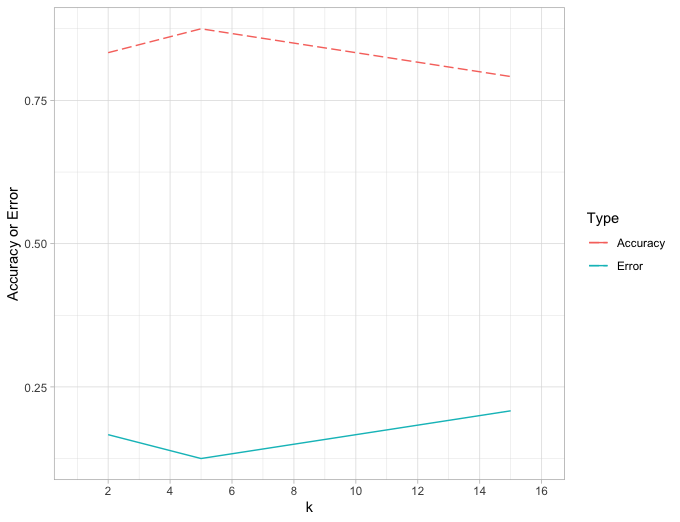
\includegraphics[width=0.8\textwidth]{HW1_3.png}
\end{figure}

We can see that the accuracy is the highest when K=5, but the differences between these three K's values are not significant. Meanwhile, the results has a close relationship with the random selection of the 10 genes. Different selected genes will lead to different results. Maybe the accuracy reach the best in $K=2$ or $K=15$ with using other 10 genes.

\end{document}